\documentclass{article}

\usepackage{arxiv}         % color.jpg palette; use [print] for grayscale on white

\usepackage{fontspec}       % load system fonts under XeLaTeX
\usepackage{hyperref}       % hyperlinks
\usepackage{url}            % simple URL typesetting
\usepackage{booktabs}       % professional-quality tables
\usepackage{amsfonts}       % blackboard math symbols
\usepackage{nicefrac}       % compact symbols for 1/2, etc.
\usepackage{microtype}      % microtypography
\usepackage{cleveref}       % smart cross-referencing
\usepackage{lipsum}         % Can be removed after putting your text content
\usepackage{graphicx}
\usepackage{pgfplots}       % editable example chart; omit if not needed
\pgfplotsset{compat=1.18}
\usepackage{natbib}
\usepackage{doi}

\title{A template for the \emph{arxiv} style}

% Here you can change the date presented in the paper title
%\date{September 9, 1985}
% Or remove it
%\date{}

\author{%
	Flowers for Tuesday \\
	Raya Lucaria Academy\\
	\texttt{flowersfortuesday@gmail.com} \\
}

% Leave the running header empty; remove the notice under the title.
\renewcommand{\headeright}{}
\renewcommand{\undertitle}{}
\renewcommand{\shorttitle}{}

% Optional cover details; title, authors and date are reused automatically.
\coverlabel{A Preprint}
\coversubtitle{Notes on research and discovery}
\covernote{}
% The icon is exclusive to the cover; keep the author text centered.
\covericon{%
	\makebox[0pt][r]{%
		\href{https://flowersfortuesday.com}{%
			\raisebox{-0.25em}{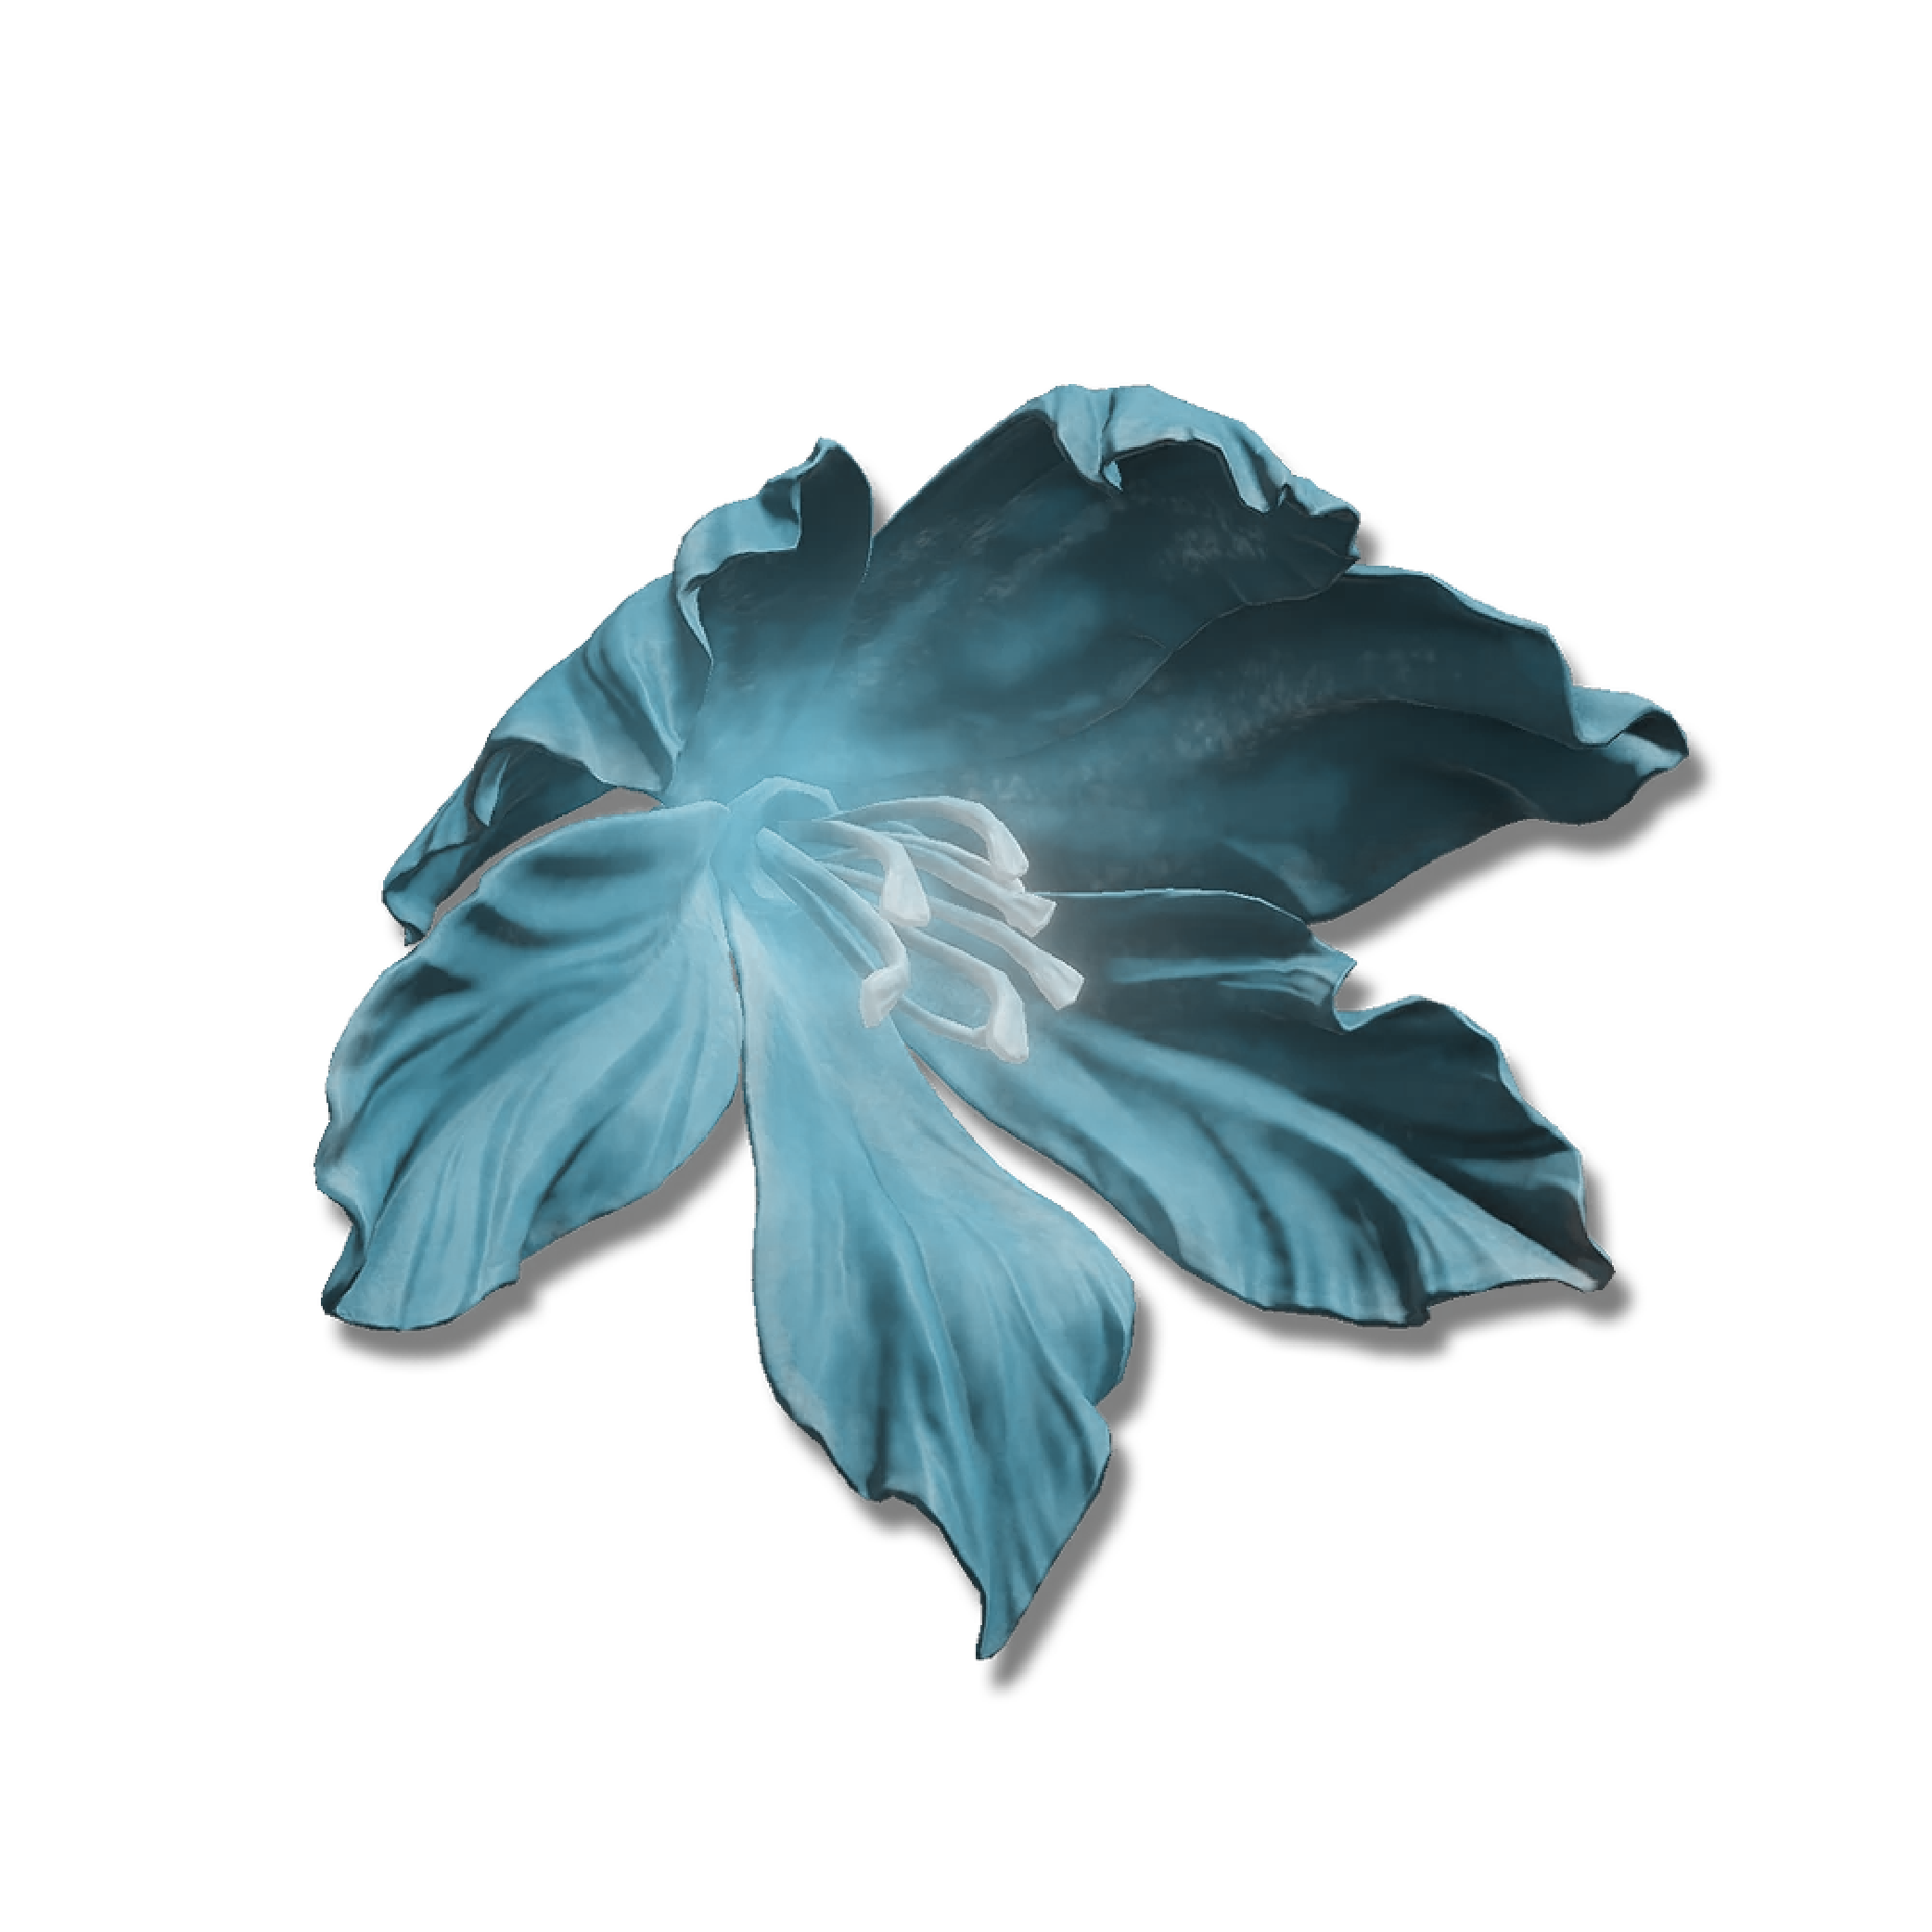
\includegraphics[height=1.35em]{icon.pdf}}}%
		\hspace{0.35em}}%
}

%%% Add PDF metadata to help others organize their library
%%% Once the PDF is generated, you can check the metadata with
%%% $ pdfinfo template.pdf
\hypersetup{
pdftitle={A template for the arxiv style},
pdfsubject={q-bio.NC, q-bio.QM},
pdfauthor={Flowers for Tuesday},
pdfkeywords={First keyword, Second keyword, More},
}

\begin{document}
\makecover % Remove this line to omit the cover; article pages still start at 1.
\maketitle

\begin{abstract}
	\lipsum[1]
\end{abstract}


% keywords can be removed
\keywords{First keyword \and Second keyword \and More}


\section{Introduction}
\lipsum[2]
\lipsum[3]


\section{Headings: first level}
\label{sec:headings}

\lipsum[4] See Section \ref{sec:headings}.

\subsection{Headings: second level}
\lipsum[5]
\begin{equation}
	\xi _{ij}(t)=P(x_{t}=i,x_{t+1}=j|y,v,w;\theta)= {\frac {\alpha _{i}(t)a^{w_t}_{ij}\beta _{j}(t+1)b^{v_{t+1}}_{j}(y_{t+1})}{\sum _{i=1}^{N} \sum _{j=1}^{N} \alpha _{i}(t)a^{w_t}_{ij}\beta _{j}(t+1)b^{v_{t+1}}_{j}(y_{t+1})}}
\end{equation}

\subsubsection{Headings: third level}
\lipsum[6]

\paragraph{Paragraph}
\lipsum[7]



\section{Examples of citations, figures, tables, references}
\label{sec:others}

\subsection{Citations}
Citations use \verb+natbib+. The documentation may be found at
\begin{center}
	\url{http://mirrors.ctan.org/macros/latex/contrib/natbib/natnotes.pdf}
\end{center}

Here is an example usage of the two main commands (\verb+citet+ and \verb+citep+): Some people thought a thing \citep{kour2014real, keshet2016prediction} but other people thought something else \citep{kour2014fast}. Many people have speculated that if we knew exactly why \citet{kour2014fast} thought this\dots

\subsection{Figures}
\lipsum[10]
See Figure \ref{fig:fig1}. Here is how you add footnotes. \footnote{Sample of the first footnote.}
\lipsum[11]

\begin{figure}
	\centering
	% Illustrative data only. Replace the values or use \includegraphics.
	\begin{tikzpicture}
		\begin{axis}[
			width=11cm, height=5.5cm,
			ybar, bar width=32pt, bar shift=0pt,
			xmin=-0.6, xmax=3.6, ymin=0, ymax=100,
			xtick={0,1,2,3},
			xticklabels={Baseline,Variant A,Variant B,Proposed},
			ytick={0,25,50,75,100}, ylabel={Score (\%)},
			axis background/.style={fill=paperSurface},
			axis line style={draw=paperSage},
			axis x line*=bottom, axis y line*=left,
			ymajorgrids=true, grid style={draw=paperLine},
			tick style={draw=paperSage},
			tick label style={font=\small, text=paperInk},
			label style={font=\small, text=paperInk},
			nodes near coords,
			every node near coord/.append style={font=\small, text=paperInk},
		]
			\addplot[fill=paperAlmond, draw=paperForest] coordinates {(0,58)};
			\addplot[fill=paperMatcha, draw=paperForest] coordinates {(1,72)};
			\addplot[fill=paperForest, draw=paperForest] coordinates {(2,81)};
			\addplot[fill=paperEclipse, draw=paperEclipse] coordinates {(3,89)};
		\end{axis}
	\end{tikzpicture}
	\caption{Illustrative comparison using almond, matcha, forest, and eclipse tones. Values are sample data, not experimental results.}
	\label{fig:fig1}
\end{figure}

\subsection{Tables}
See awesome Table~\ref{tab:table}.

The documentation for \verb+booktabs+ (`Publication quality tables in LaTeX') is available from:
\begin{center}
	\url{https://www.ctan.org/pkg/booktabs}
\end{center}


\begin{table}
	\caption{Sample table title}
	\centering
	\begin{tabular}{lll}
		\toprule
		\multicolumn{2}{c}{Part}                   \\
		\cmidrule(r){1-2}
		\rowcolor{paperForest}
		\textcolor{paperBackground}{\bfseries Name}
		         & \textcolor{paperBackground}{\bfseries Description}
		                           & \textcolor{paperBackground}{\bfseries Size ($\mu$m)} \\
		\midrule
		\rowcolor{paperSurface}
		Dendrite & Input terminal  & $\sim$100     \\
		\rowcolor{paperMatcha!12!paperBackground}
		Axon     & Output terminal & $\sim$10      \\
		\rowcolor{paperSurface}
		Soma     & Cell body       & up to $10^6$  \\
		\bottomrule
	\end{tabular}
	\label{tab:table}
\end{table}

\subsection{Lists}
\begin{itemize}
	\item Lorem ipsum dolor sit amet
	\item consectetur adipiscing elit.
	\item Aliquam dignissim blandit est, in dictum tortor gravida eget. In ac rutrum magna.
\end{itemize}


\bibliographystyle{unsrtnat}
\bibliography{references}  %%% Uncomment this line and comment out the ``thebibliography'' section below to use the external .bib file (using bibtex) .


%%% Uncomment this section and comment out the \bibliography{references} line above to use inline references.
% \begin{thebibliography}{1}

% 	\bibitem{kour2014real}
% 	George Kour and Raid Saabne.
% 	\newblock Real-time segmentation of on-line handwritten arabic script.
% 	\newblock In {\em Frontiers in Handwriting Recognition (ICFHR), 2014 14th
% 			International Conference on}, pages 417--422. IEEE, 2014.

% 	\bibitem{kour2014fast}
% 	George Kour and Raid Saabne.
% 	\newblock Fast classification of handwritten on-line arabic characters.
% 	\newblock In {\em Soft Computing and Pattern Recognition (SoCPaR), 2014 6th
% 			International Conference of}, pages 312--318. IEEE, 2014.

% 	\bibitem{keshet2016prediction}
% 	Keshet, Renato, Alina Maor, and George Kour.
% 	\newblock Prediction-Based, Prioritized Market-Share Insight Extraction.
% 	\newblock In {\em Advanced Data Mining and Applications (ADMA), 2016 12th International 
%                       Conference of}, pages 81--94,2016.

% \end{thebibliography}


\end{document}
